\begin{surferPage}[99 сингуларитета]{Површ седмог реда са 99 сингуларитета}
    Радећи на својој докторској дисертацији на Универзитету у Мајнцу 2004. године, 
	Оливер Лабс је конструисао површ седмог степена са 99 сингуларитета. 
	Ово је тренутни светски рекорд за такве површи; мада је могуће да постоји површ 
	седмог степена са чак $104$ сингуларитета!  
    Лабсова површ поседује симетрију правилног $7$-угла (слика лево).
    Ово се види када се површ посматра одозго (слика десно):

    \vspace*{-0.3em}
    \begin{center}
      \begin{tabular}{c@{\qquad}c}
        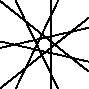
\includegraphics[height=1.5cm]{labsseptic1.pdf}
        &
        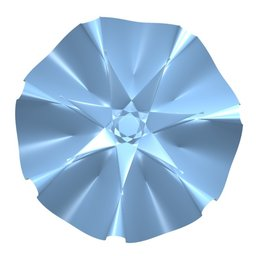
\includegraphics[height=1.5cm]{labs_septic_von_oben}
      \end{tabular}
    \end{center}
    \vspace*{-0.3em}

    Оливер Лабс је за контрукцију ове површи користио компјутерски алгебарски систем 
    SINGULAR (Универзитет у Кајзерслаутерну) који је одличан за израчунавања у 
	алгебарској геометрији и за сингуларитете.

    Он је користио чињеницу да се може рачунати са коначним скуповима бројева на 
    природан начин. Ово знамо по сатовима; 24.00$=$0.00, 24.00 $+$ 1 сат није
    25.00, већ 1.00.
\end{surferPage}
